\hfill
\center
\begin{subfigure}{\textwidth/\real{4.1}}
	\center\scalebox{0.35}{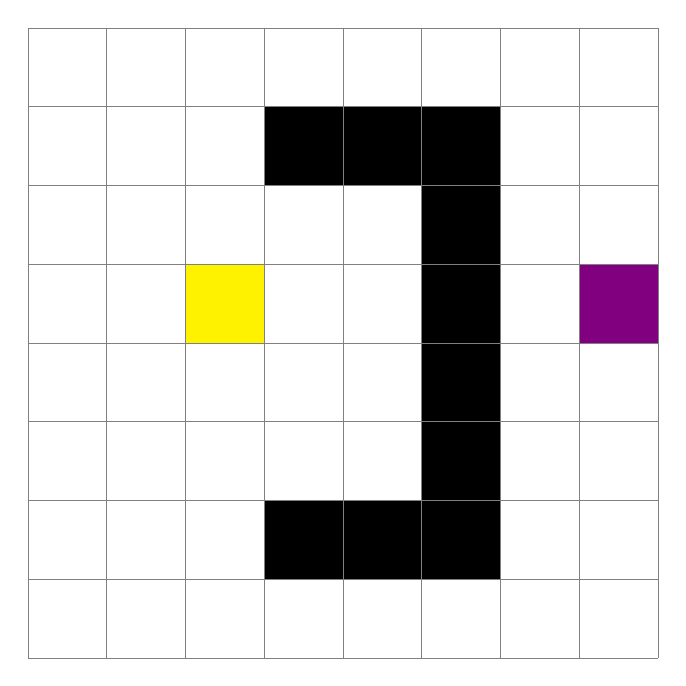
\begin{tikzpicture}
		\fill[yellow](2,4) rectangle (3,5);
		\fill[black] (3,1) rectangle (6,2);
		\fill[black] (3,6) rectangle (6,7);
		\fill[black] (5,1) rectangle (6,7);
		\fill[yellow] (2,4) rectangle (3,5);
		\fill[violet] (7,4) rectangle (8,5);
		\draw[gray,very thin] (0,0) grid (8,8);
		\end{tikzpicture}}
\end{subfigure}
\begin{subfigure}{\textwidth/\real{4.1}}
	\center\scalebox{0.35}{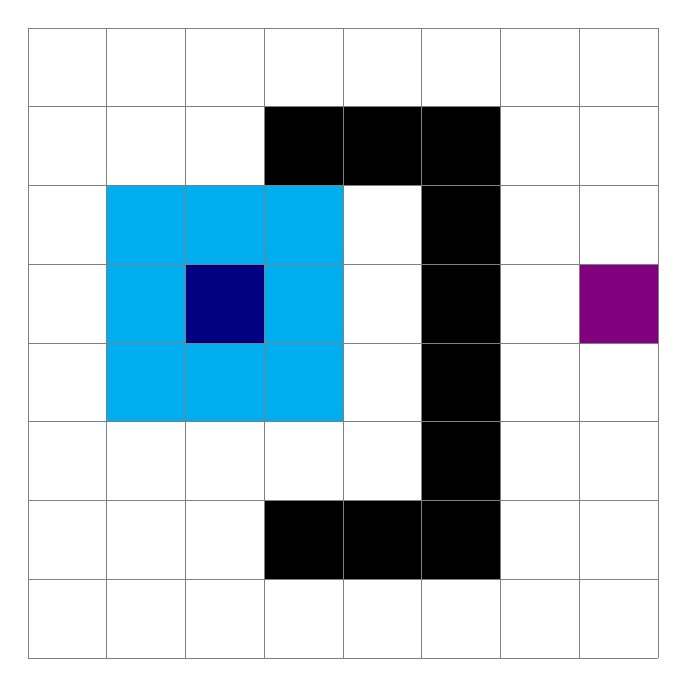
\begin{tikzpicture}
		\fill[yellow](2,4) rectangle (3,5);
		\fill[black] (3,1) rectangle (6,2);
		\fill[black] (3,6) rectangle (6,7);
		\fill[black] (5,1) rectangle (6,7);
		\fill[cyan] (1,3) rectangle (4,6);
		\fill[NavyBlue] (2,4) rectangle (3,5);
		\fill[violet] (7,4) rectangle (8,5);
		\draw[gray,very thin] (0,0) grid (8,8);
		\end{tikzpicture}}
\end{subfigure}
\begin{subfigure}{\textwidth/\real{4.1}}
	\center\scalebox{0.35}{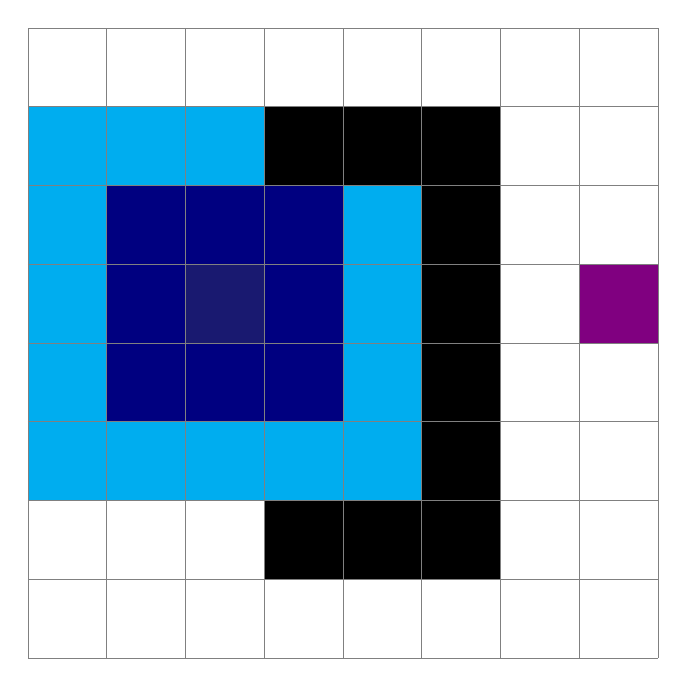
\begin{tikzpicture}
		\fill[yellow](2,4) rectangle (3,5);
		\fill[cyan] (0,2) rectangle (5,7);
		\fill[NavyBlue] (1,3) rectangle (4,6);
		\fill[MidnightBlue] (2,4) rectangle (3,5);
		\fill[black] (3,1) rectangle (6,2);
		\fill[black] (3,6) rectangle (6,7);
		\fill[black] (5,1) rectangle (6,7);
		\fill[violet] (7,4) rectangle (8,5);
		\draw[gray,very thin] (0,0) grid (8,8);
		\end{tikzpicture}}
\end{subfigure}
\hfill 